

\documentclass[
	11pt, % Set the default font size, options include: 8pt, 9pt, 10pt, 11pt, 12pt, 14pt, 17pt, 20pt
	%t, % Uncomment to vertically align all slide content to the top of the slide, rather than the default centered
	%aspectratio=169, % Uncomment to set the aspect ratio to a 16:9 ratio which matches the aspect ratio of 1080p and 4K screens and projectors
]{beamer}

\graphicspath{{~/Pictures/}{./}{./images/}} % Specifies where to look for included images (trailing slash required)

\usepackage{booktabs}% Allows the use of \toprule, \midrule and \bottomrule for better rules in tables
\usetheme{Madrid}
\usepackage{algorithm,algpseudocode}
\usefonttheme{default} % Typeset using the default sans serif font
\usepackage{palatino} % Use the Palatino font for serif text
\usepackage{amssymb}
\usepackage[default]{opensans} % Use the Open Sans font for sans serif text
\useinnertheme{circles}
\usepackage{tikz}
\usetikzlibrary{shapes.geometric, arrows}
\usepackage{hyperref}

\tikzstyle{io} = [rectangle, rounded corners, 
minimum width=3cm, 
minimum height=1cm,
text centered, 
text width=3cm,
draw=black, 
fill=red!30]

\tikzstyle{conv} = [trapezium, 
trapezium stretches=true, % A later addition
trapezium left angle=70, 
trapezium right angle=110, 
minimum width=3cm, 
minimum height=1cm, 
text centered, 
text width=3cm,
draw=black, fill=blue!30]

\tikzstyle{pool} = [rectangle, 
minimum width=3cm, 
minimum height=1cm, 
text centered, 
text width=3cm, 
draw=black, 
fill=orange!30]

\tikzstyle{fc} = [ellipse, 
minimum width=3cm, 
minimum height=1cm, 
text centered, 
text width=3cm,
draw=black, 
fill=green!30]
\tikzstyle{arrow} = [thick,->,>=stealth]

\title[Logistic Map]{The Logistic Map}
\subtitle{A Journey into Chaos}

%subtitle{Exploring CNNs for Space Object Classification} % Presentation subtitle, remove this command if a subtitle isn't required

\author[Cotton]{Nicholas Cotton} % Presenter name(s), the optional parametercan contain a shortened version to appear on the bottom of every slide, while the main parameter will appear on the title slide
\date[\today]{\today} % Presentation date or conference/meeting name, the optional parameter can contain a shortened version to appear on the bottom of every slide, while the required parameter value is output to the title slide
\begin{document}
\begin{frame}
	\titlepage % Output the title slide, automatically created using the text entered in the PRESENTATION INFORMATION block above
\end{frame}
\begin{frame}
	\frametitle{Presentation Overview} % Slide title, remove this command for no title
	
	\tableofcontents % Output the table of contents (all sections on one slide)
	%\tableofcontents[pausesections] % Output the table of contents (break sections up across separate slides)
\end{frame}
\section{Introduction} % Sections are added in order to organize your presentation into discrete blocks, all sections and subsections are automatically output to the table of contents as an overview of the talk but NOT output in the presentation as separate slides
\subsection{What is Logistic map?}

\begin{frame}
	\frametitle{What is the Logistic map?}
 \begin{block}{The Logistic Map}
     The Logistic Map is a function $f:[0,1]\to[0,1]$ defined  as
     \[f(x)=rx(1-x)\]
     or more commonly
     \[x_{n+1}=rx_n(1-x_n)\]
     where
     \begin{itemize}
         \item $x_n$ is the (normalized) population at a time $n$
         \item $r$ is a parameter that controls the rate of population growth. Here we focus on $0\leq r\leq 4$
     \end{itemize}
 \end{block}
 
 \begin{itemize}
 
     \item 
     	Note that the Logistic Map consists of a growth term $rx_n$ and a limiting factor $(1-x_n)$
      
 \end{itemize}

 

\end{frame}
\subsection{Just a parabola?}
\begin{frame}
	\frametitle{Just a parabola?}
 		You might notice that the Logistic Map is just a quadratic of form $f(x)=rx-rx^2$
	\begin{itemize}
		\item
  The graph of a single iteration is simply a parabola, regardless of initial conditions
        \item 
        We can clearly see that this achieves its maximum value at $x_{max}=\frac{1}{2}$
        \begin{itemize}
            \item Plugging in $x_{max}$, we can see that the maximum value is $\frac{r}{4}$
            \item This explains why we focus on $0\leq r\leq 4$
        \end{itemize}

	\end{itemize}
	\begin{figure}
	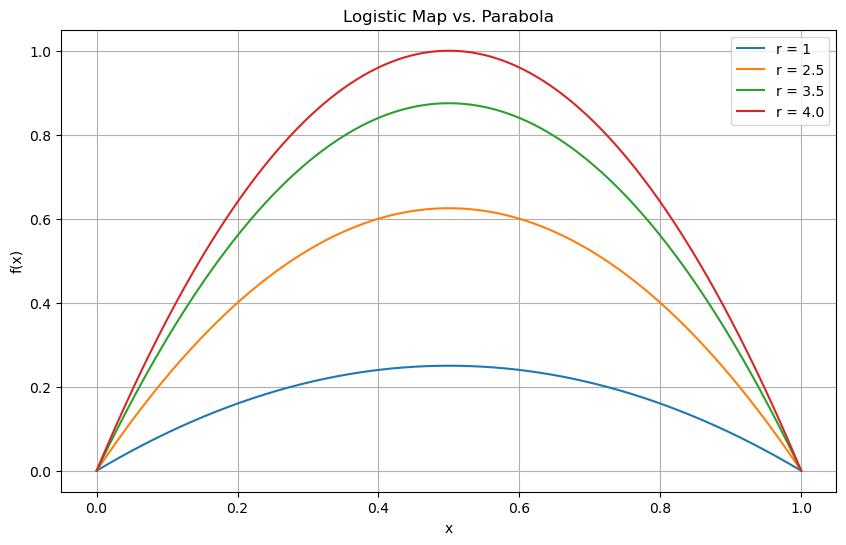
\includegraphics[scale=0.25]{./figures/parabolas}
	\end{figure}
\end{frame}
\section{Stability and Bifurcation Analysis}
\begin{frame}
	\frametitle{Long Term Behaviors}
 \begin{itemize}
     \item 
     	Of course, this is a dynamical system, so we are interested in the \emph{long term} behavior of the map
      \item 
        We do this by fixing $r$ and seeing what sort of behaviors occur after iterating the map many times
        \begin{itemize}
            \item Fixed and periodic points
            \item Stability at those points
            \item Denseness of orbits
            \item Chaos?
        \end{itemize}
 \end{itemize}
 	\begin{figure}
	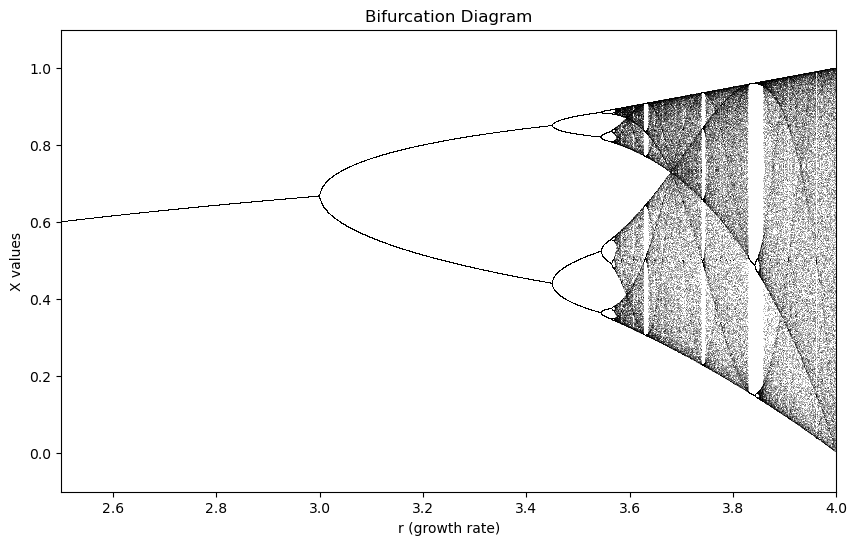
\includegraphics[scale=0.3]{./figures/bifurcations}
	\end{figure}
 
\end{frame}
\subsection{Stability of Fixed/Periodic Points}
\begin{frame}{Stability of Fixed/Periodic Points}
For various distinct regions of $r$, we want find fixed/periodic points and study their stability.
\begin{block}{Checking stability of a point}
\begin{enumerate}
    \item
    We first consider the first order Taylor Series expansion around a fixed or periodic point $x^\ast$
    \[x_{n+1}=f'(x^\ast)(x_n-x^\ast)+x^\ast\]
    where $f'(x^\ast)$ is the derivative of the Logistic Map at $x^\ast$.
    \begin{itemize}
        \item $f'(x^\ast)=r(1-2x^\ast)$
    \end{itemize}
    \item
        We say that $x^\ast$ is \emph{stable} if $|f'(x^\ast)|<1$ since this means that points around $x^\ast$ will converge to $x^\ast$.
\end{enumerate}
    
\end{block}
\end{frame}
\begin{frame}{$r<1$}
Note that we have an obvious fixed point at $x^\ast=0$.
\begin{itemize}
    \item Taking the derivitive gives us 
    \[f'(x^\ast)=r(1-2x^\ast)=r\]
    \item
    Since $r<1$, $|r|<1$ and so $x^\ast=0$ is a stable fixed point.
    \item
	    We also see convergence to $0$ in the $r=1$ case
\end{itemize}
 	\begin{figure}
	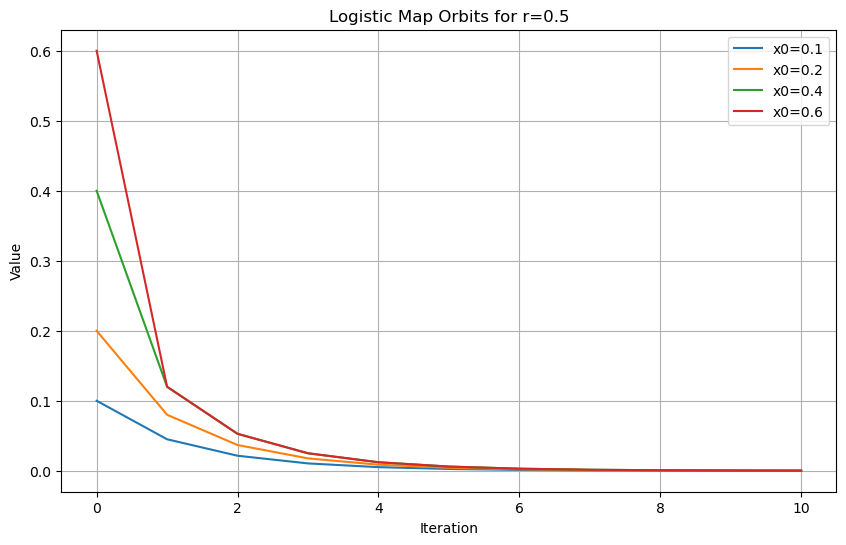
\includegraphics[scale=0.3]{./figures/rles1}
	\end{figure}
\end{frame}
\begin{frame}{$1 < r<2$}
When $1< r<2$, we still have our fixed point at 0; however, checking for stability shows
\[|f'(0)|=|r|> 1\]
Thus, $0$ is not a stable fixed point. 

Checking for other fixed points, we find one at $x^\ast=\frac{r-1}{r}$

\begin{itemize}
    \item This time
    \[f'(x^\ast)=r(1-2x^\ast)=\frac{2-r}{r}\]
    \item 
    Clearly, $|f'(x^\ast)|<1$ and so $x^\ast=\frac{r-1}{r}$ is a stable fixed point.
     	\begin{figure}
	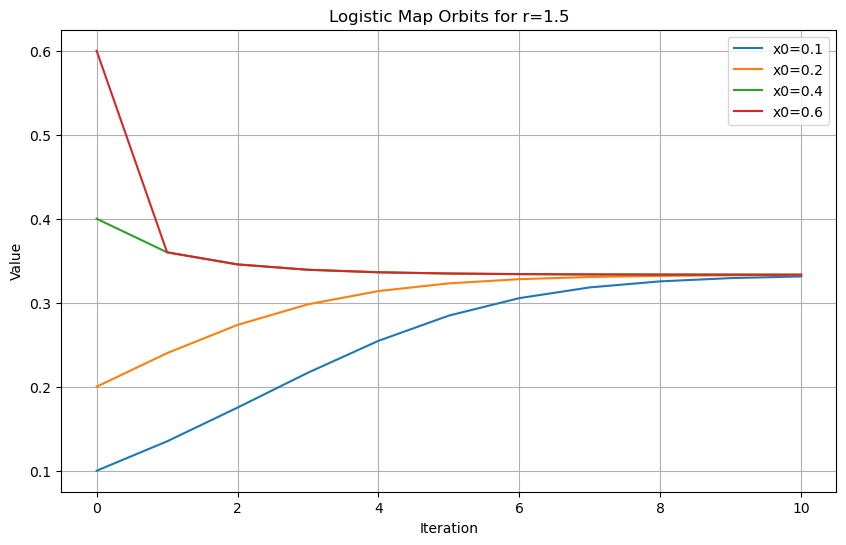
\includegraphics[scale=0.25]{./figures/1lesrles2}
	\end{figure}
\end{itemize}
    
\end{frame}
\begin{frame}{$2\leq r<3$}
\begin{itemize}
    \item For this case we perform the same analysis for $x^\ast=\frac{r-1}{r}$
    \item $|f'(x^\ast)|$ is still less than 1
    \item However, in this region of $r$, while no points are periodic (except the fixed point), we see some oscillations before converging to $x^\ast$
    \begin{itemize}
        \item This hints at possible periodicity in other regions of $r$
    \end{itemize}
\end{itemize}
     	\begin{figure}
	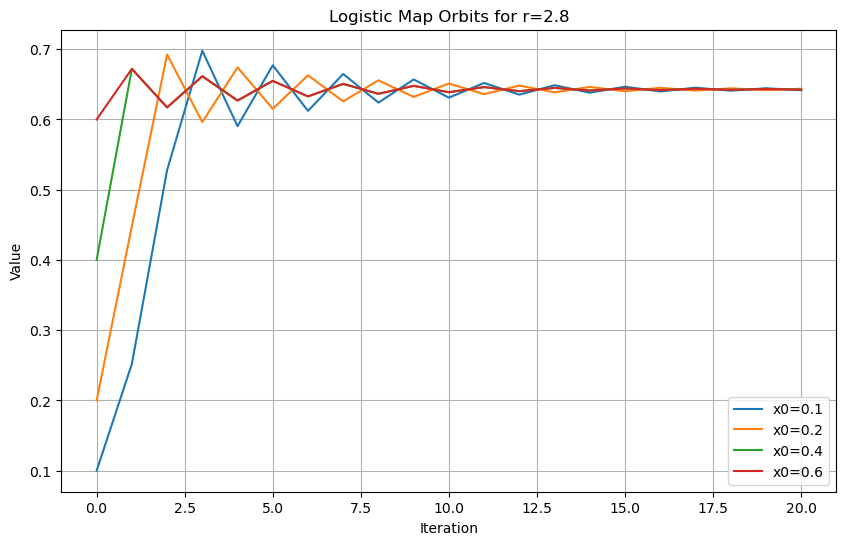
\includegraphics[scale=0.3]{./figures/2lesrles3}
	\end{figure}
\end{frame}
\begin{frame}{$3\leq r<4$}
\begin{itemize}
    \item This is where things get interesting
    \item We see many different behaviors in this region of $r$
    \item For $3\leq r<1+\sqrt{6}$ we have 2 stable periodic points at
    \[x_{\pm}=\frac{1}{2r}(r+1\pm\sqrt{(r-3)(r+1)})\]
     	\begin{figure}
	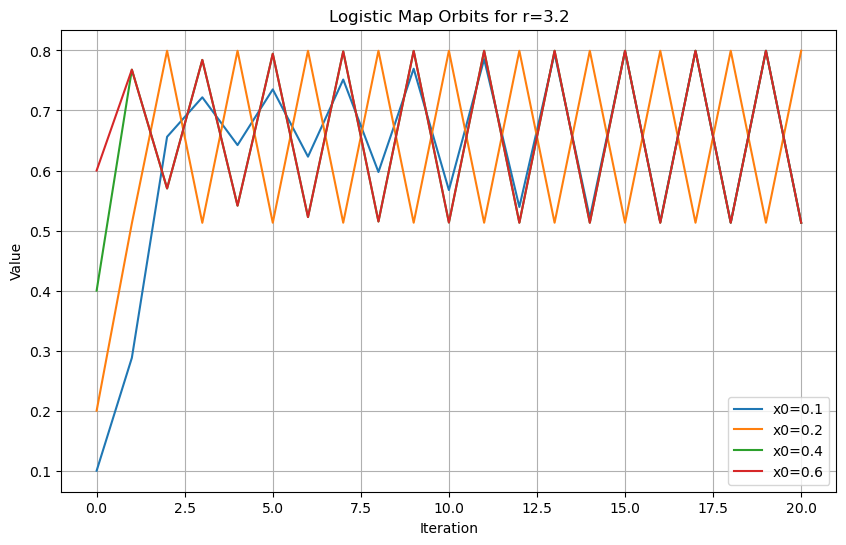
\includegraphics[scale=0.3]{./figures/period2}
	\end{figure}
\end{itemize}
    
\end{frame}
\begin{frame}{$3\leq r<4$}
Immediately after $r=1+\sqrt{6}$ we find period 2 orbits, then period 4 orbits, then period 8 orbits and so on...
\begin{itemize}
\item 
This period doubling continues until we reach $r\approx 3.56995$
\begin{itemize}
    \item This region of $3\leq r< 3.56995$ is commonly referred to as the \emph{period doubling cascade}
\end{itemize}
\item $r>3.56995$ is characterized by chaotic behavior
\end{itemize}
\end{frame}
\subsection{Bifurcation Diagram}
\begin{frame}{Bifurcation Diagram}
The bifurcation diagram is an interesting numerical result that helps us visualize the change in behavior across different values of $r$

\begin{block}{Generating the diagram}
\begin{enumerate}
    \item Fix $x_0$
    \item Iterate the map $1000$ times to ensure we are looking at long term behavior
    \item Plot the next $100$ iterations
    \item Repeat 2-3 for each value of $r$
\end{enumerate}
\end{block}
\end{frame}
\begin{frame}{Bifurcation Diagram}
     	\begin{figure}
	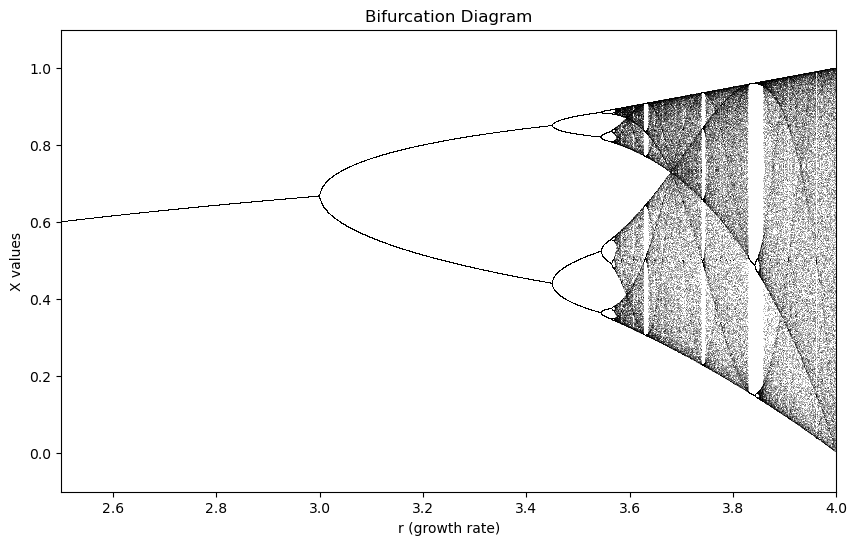
\includegraphics[scale=0.5]{./figures/bifurcations}
	\end{figure}
    
\end{frame}
\section{Chaos}
\begin{frame}{Chaos}
    \begin{itemize}
        \item In this context we define Chaos as satisfying the following conditions
        \begin{enumerate}
            \item Sensitive dependence on initial conditions
            \item Topological Mixing
            \item Dense orbits
        \end{enumerate}
        \item For logistic map, we look at the region $r>3.56995$ as showing chaotic behavior.
        \end{itemize}
        \begin{figure}
	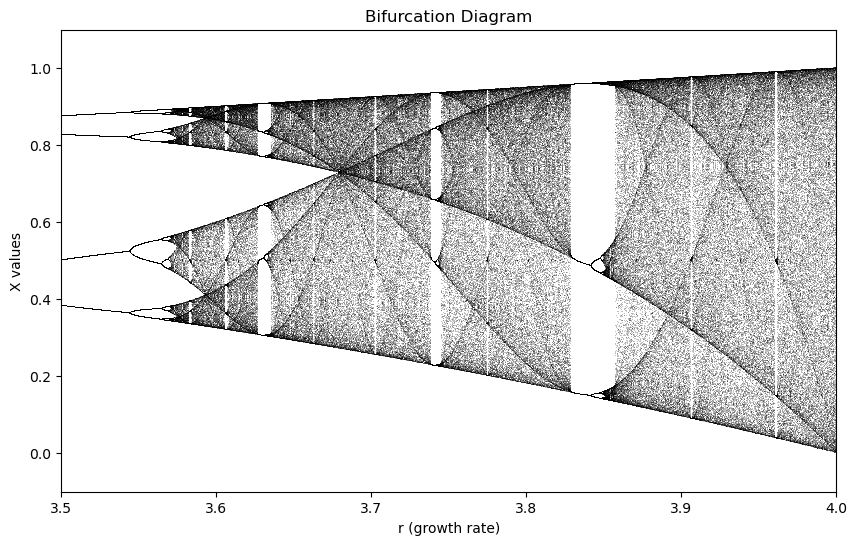
\includegraphics[scale=0.3]{./figures/chaosregion}
	\end{figure}
\end{frame}
\subsection{Randomness vs. Chaos}
\begin{frame}{Randomness vs. Chaos}
\begin{itemize}
    \item Plotting logistic map orbits in this region against random data may lead us to believe that the orbits in this region are completely random
    \item However, the orbit of a point is entirely determined by its initial conditions.
    \item Plotting $x_{n}$ against $x_{n+1}$ in whats known as a \emph{Poincare plot}, the logistic map shows behavior determined entirely by the equation itself while the random data just looks like noise
\end{itemize}

\begin{figure}
    \centering
    \begin{minipage}{0.45\textwidth}
        \centering
        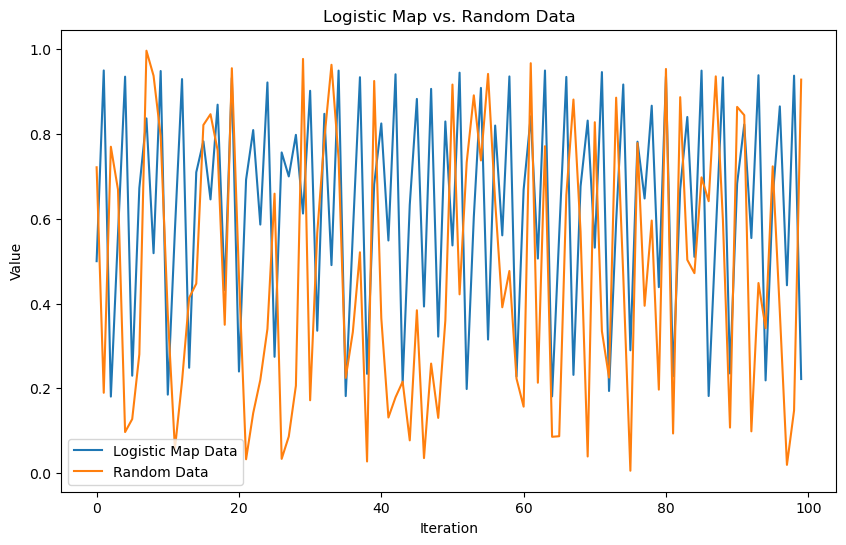
\includegraphics[width=0.9\textwidth]{./figures/logvsrand.png}% first figure itself

    \end{minipage}\hfill
    \begin{minipage}{0.3\textwidth}
        \centering
        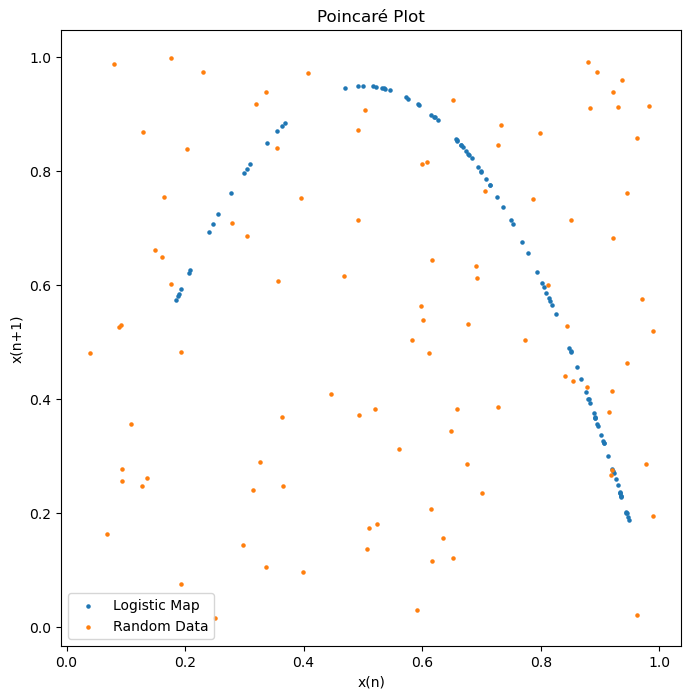
\includegraphics[width=0.9\textwidth]{./figures/Poincare} % second figure itself
    \end{minipage}
            \caption{Generated with $x_0=0.5$ and $r=3.8$}
\end{figure}
\end{frame}
\subsection{Sensitive dependence on Initial Conditions}
\begin{frame}{Sensitive Dependence on Initial Conditions}

\begin{block}{Sensitive Dependance on Initial Conditions}
    For any two initial values $x_0$ and $x'_0$, the distance between their orbits grows exponentially. More specifically, there exists $\lambda>0$ s.t.
    \[|x_n-x'_n| = e^{\lambda n}|x_0-x'_0|\]
    $\lambda$ is called Lyapunov Exponent
\end{block}
        \begin{figure}
	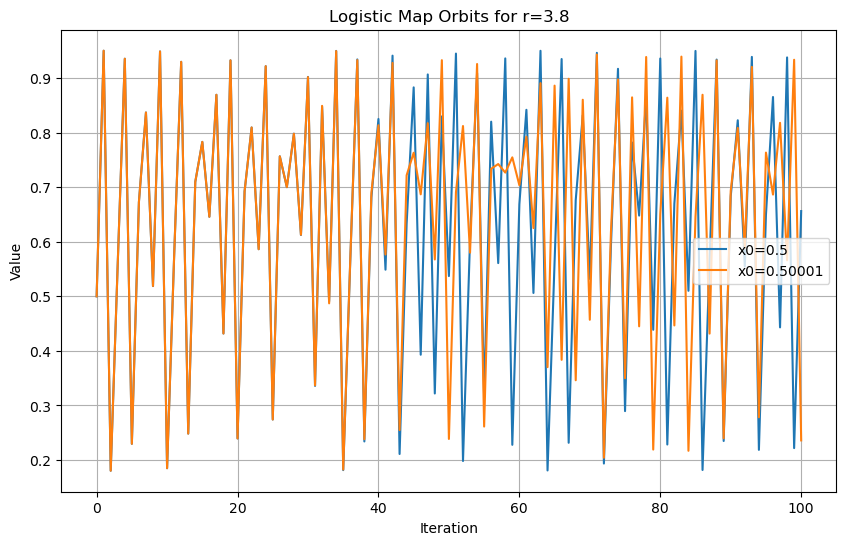
\includegraphics[scale=0.3]{./figures/sensitivity}
	\end{figure}

    
\end{frame}
\subsubsection{Lyapunov Exponents}
\begin{frame}{Lyapunov Exponents}
Lyapunov Exponents measure how quickly initially nearby points diverge.
\begin{itemize}
    \item A positive Lyapunov Exponent indicates exponential divergence
    \item A negative Lyapunov Exponent indicates exponential convergence.
    \item Computed using:
    \[\lambda=\lim_{n\to\infty}\frac{1}{n}\sum^n_{i=1}\ln|f'(x_i)|\]
\end{itemize}
\end{frame}
\subsection{Topological Mixing and Dense Orbits}
\begin{frame}{Topological Mixing}
\begin{block}{Topological Mixing}
    A map $f:X\to X$ is topologically mixing if for any non-empty open sets $U,V\subseteq X$,
    \[f^n(U)\cap V\neq \emptyset\]
    for sufficiently large $n$.
\end{block}
\begin{itemize}
    \item This can easily be proven for $r=4$.
    \begin{enumerate}
        \item Define semi-conjugacy with $E_2(x)=2x\mod 1$ by $h=\sin^2\pi x$
        \item Take orbits of logistic map to orbits of $E_2$
        \item We have already proved $E_2$ is Topologically Mixing in Class
    \end{enumerate}   
    \end{itemize}
    
\end{frame}
\begin{frame}{Dense Orbits}
\begin{block}{Dense Orbits}
	A point has orbit dense in $[0, 1]$ if it visits every
	open interval in $[0,1]$.
\end{block}
\begin{itemize}
	\item
		Here we can see this property for the case of $r=4$.
\end{itemize}
        \begin{figure}
	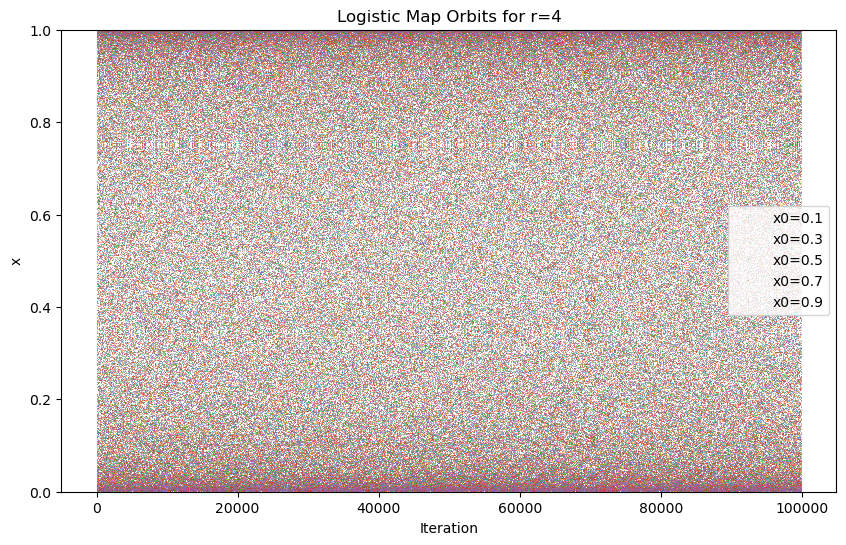
\includegraphics[scale=0.2125]{../figures/denseorbits.png.png}
	\end{figure}
\end{frame}
\subsection{Stable Period-3 Orbit Emerges!}
\begin{frame}{Stable Period-3 Orbit Appears!}
    \tikz[remember picture, overlay] {\node[anchor=south east, outer sep=0pt] at (current page.south east) {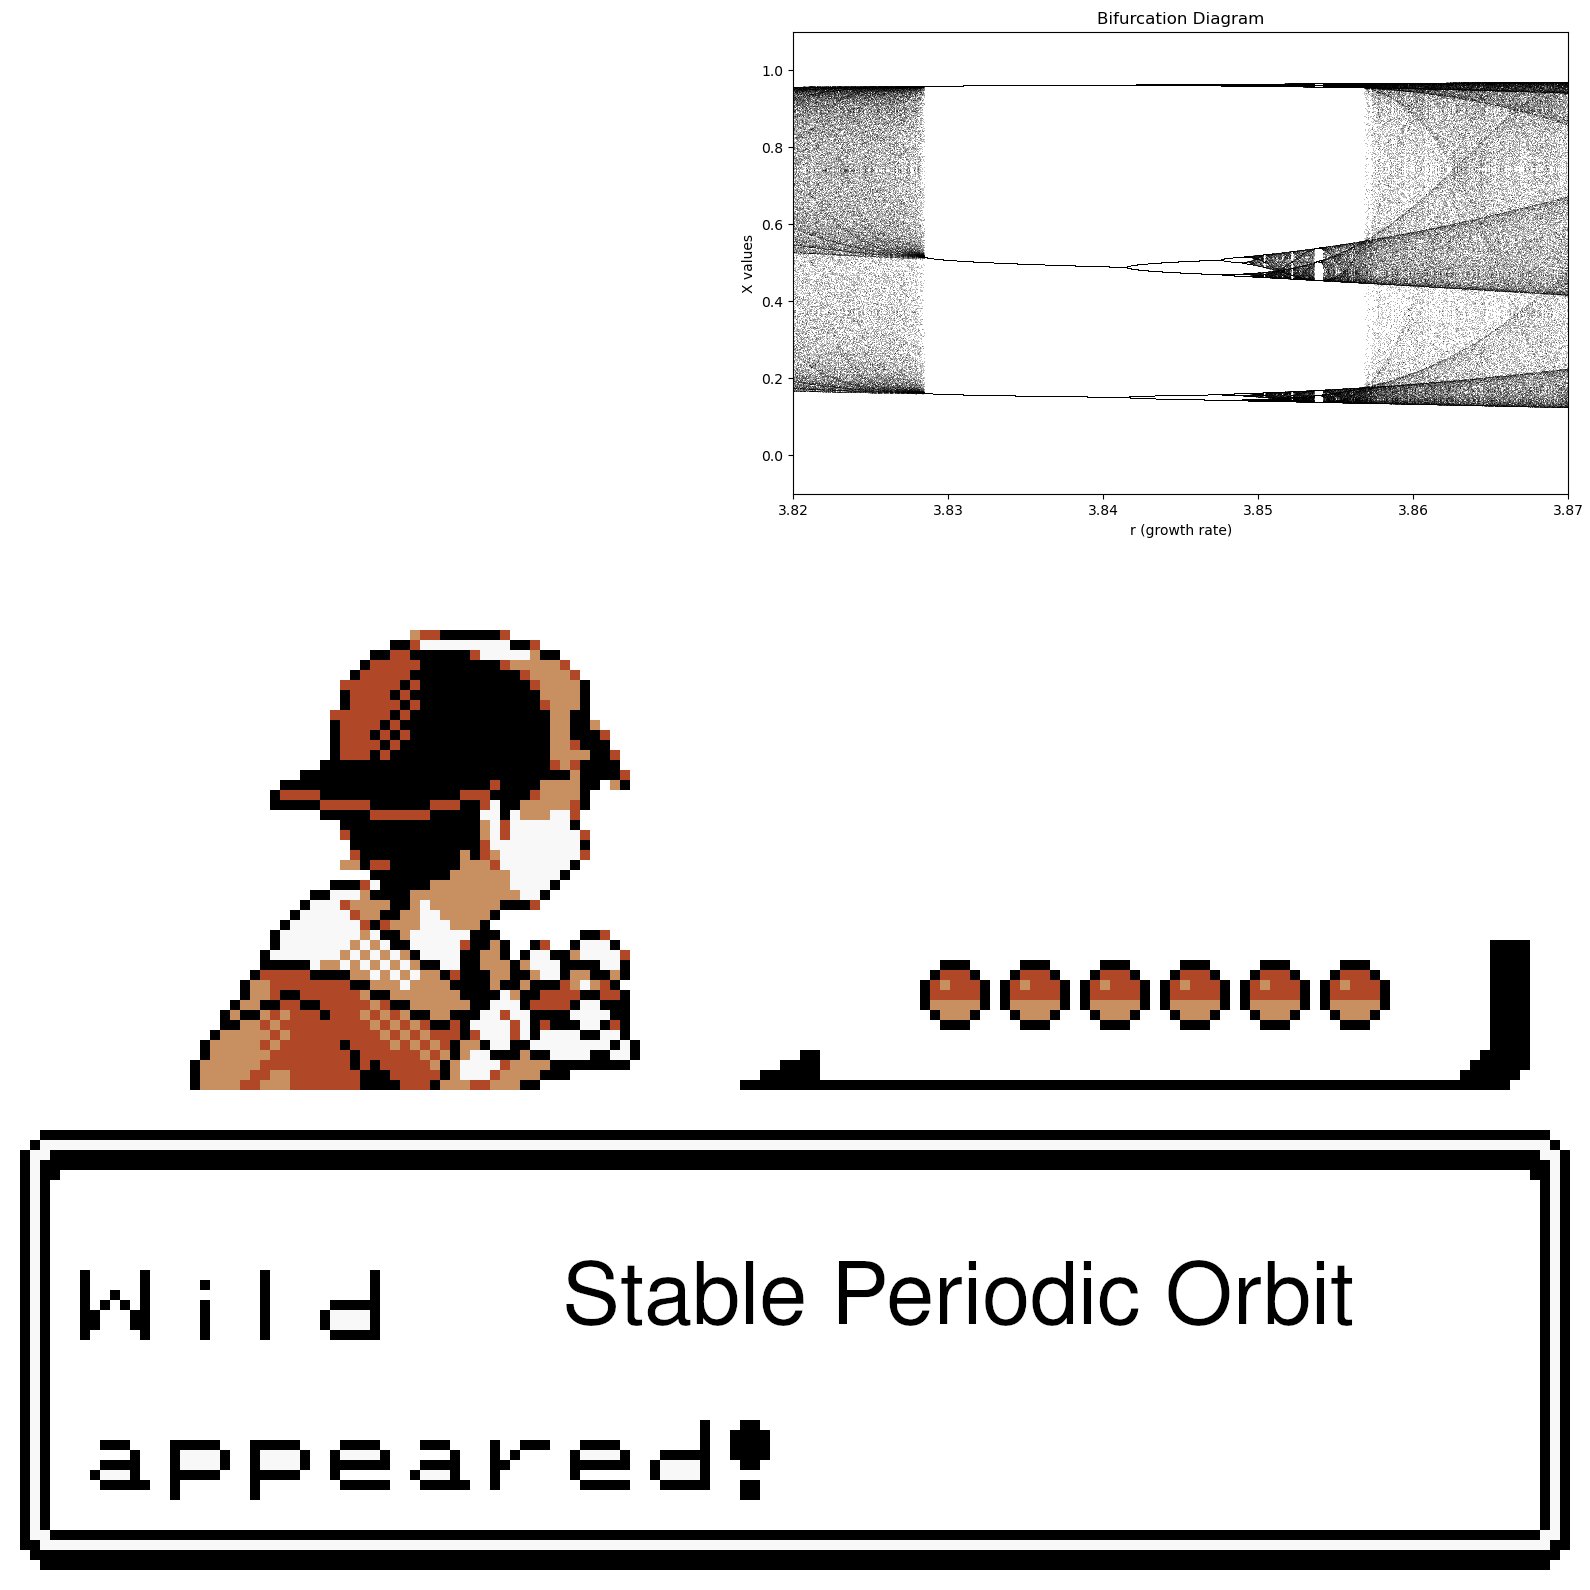
\includegraphics[width=5cm]{./figures/pokep3}};}
    Remarkably, suddenly at $r=1+\sqrt{8}$, three stable period-3 periodic points appear. 
    \begin{itemize}
        \item We can check the Lyapunov Exponents in this region and see that they are negative
        \item We can see this on the bifurcation diagram
        \item We see period doubling before quickly
        
        returning to chaos
    \end{itemize}
\end{frame}
\section{Attractors and Fractals}
\subsection{Attractors}
\begin{frame}{Attractors}
On the bifurcation diagram, we can see that chaotic orbits, while not converging to periodic points, still remain in some bounded region after many iterations
\begin{itemize}
    \item This region is called an attractor
\end{itemize}
\begin{block}{Attractor} 
For a function $f:X\to X$, a attractor is a subset $A$ of $X$ s.t
\begin{enumerate}
	\item $a\in A\implies f^n(a)\in A$ for all $n\in\mathbb{N}$
    \item There exists a neighborhood of A, denoted $B(A)$, defined as the set of all $b\in X$ s.t. for any open set $V$ containing $A$, $g^n(b)\in V$ for sufficiently large $n$.
    \item There is no smaller subset of $A$ satisfying $(1)$ and $(2)$
\end{enumerate}
\end{block}



\end{frame}
\subsection{Video}
\begin{frame}{Video}

\url{https://youtu.be/PtfPDfoF-iY?si=NTYnzAEWu-ngK0pb}
    
\end{frame}
\end{document} 
